\subsection*{\large{Выбор архитектуры системы}}
\addcontentsline{toc}{subsection}{Выбор архитектуры системы}

Для решения задачи автоматической генерации генерального плана сооружения предлагается следующая архитектура системы.

\begin{figure}[H]
	\hspace*{-2.5 cm}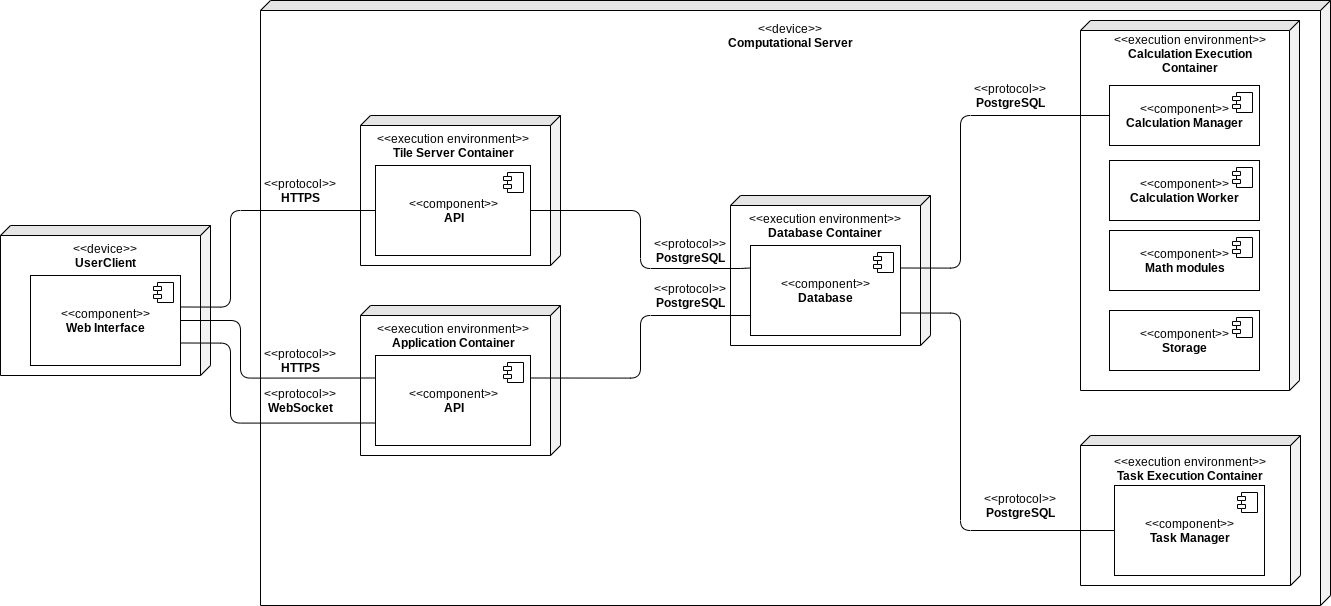
\includegraphics[width=1.2\textwidth, left]{images/architecture/1}
	\caption{Диаграмма размещения}
	\label{pic:architecture__deployment-diagram}
\end{figure}
\vskip 5 mm

\noindent Компоненты представленные на диаграмме:
\begin{itemize}
	\item \textbf{Web Interface} -- веб-интерфейс, позволяющий осуществлять взаимодействие с системой пользователю.
	\item \textbf{Tile Server Container}
	\begin{itemize}
		\item API -- веб-сервер, предоставляеющий API для получения подложки карты.
	\end{itemize}
	\item \textbf{Application Container}
	\begin{itemize}
		\item API -- веб-сервер, предоставляющий GraphQL-API для взаимодействия с системой.
		Также отвечает за предоставление и обработку данных, обеспечивающих выполнение расчета.
	\end{itemize}
	\item \textbf{Database} -- база данных, используемая для хранения данных расчетных задач.
	\item {\bf Task Execution Container}
	\begin{itemize}
		\item Task Manager -- компонент, контролирующий расчет задачи. Последовательно вызывает этапы выполнения задачи.
	\end{itemize}
	\item {\bf Calculation Execution Container}
	\begin{itemize}
		\item Calculation Manager -- компонент, осуществляющий получение и преобразование данных задачи из БД к задачам,
		обрабатываемых Calculation Worker-ами, а также за запуск Computational Worker-ов.
		\item Calculation Worker -- компонент, осуществляющий запуск метода в отдельном процессе, обработку и сохранение решения.
		\item Math Modules -- модули, представляющие собой математические библиотеки, которые могут быть использованы Computational Worker-ом.
		\item Storage -- компонент, осуществляющий чтение/запись входных данных для метода.
	\end{itemize}
\end{itemize}


Расчет генплана площадного объекта -- это комплексная задача, которая состоит из множества различных,
связанных между собой этапов. Результатом задачи является построенный генеральный план.
Генеральный план состоит из следующих объектов:
\begin{itemize}
	\item Местоположение сооружений.
	\item Коммуникационные сети (линии электропередач, трубопроводы).
	\item Эстакады для прокладки коммуникационных сетей.
	\item Внутриплощадочные проезды.
	\item Местоположение площадного объекта на местности.
	\item Зоны теплового излучения.
	\item Зоны поражения взрывных волн.
	\item Объёмы выемки/отсыпки строительной площадки.
	\item Ограждения групп сооружений.
\end{itemize}

Вычисление всех этих объектов представляет последовательный вызов расчетных методов.
Каждый из этих методов выполняет свою определенную задачу: один рассчитывает местоположения зданий, другой, на основе
местоположений зданий рассчитывает конфигурацию внутриплощадочных проездов. Каждый из методов влияет на
результаты других методов. Поэтому разная последовательность их вызовов может давать кардинально разные результаты.

Расчет каждого метода может продолжаться длительное время (например: больше одного часа). Поэтому очень важно
рассматривать расчет задачи именно исходя из методов, так как существуют различные методики для расчета



